\documentclass[14pt,a4paper]{article}

\usepackage[utf8]{inputenc}
\usepackage[english,russian]{babel}
\usepackage[T2A]{fontenc}
\usepackage{graphicx}
\usepackage{amssymb}
\usepackage{amsthm}
\usepackage{bm}
\graphicspath{{media}}
\usepackage{float}
\usepackage{}
%\setlength{\parindent}{1.25cm}
\usepackage{indentfirst}
\usepackage[a4paper,
%showframe, % отображение границ области листа
top		=	2.00cm,
bottom	=	2.00cm,
left	=	3.00cm,
right	=	1.50cm,
nohead,
foot	=	0.75cm
]{geometry} % пакет формата листа

\setlength{\parindent}{1.25cm} % задаём размер красной строки
\usepackage{setspace} % пакет для работы с интервалами
\onehalfspacing % полуторный интервал

\begin{document}
    \section*{Введение.}
    
    Клапан Тесла - это обратный клапан, в котором отсутствуют механические подвижны части. Клапаны такого типа обладают такими преимуществами как масштабируемость, долговечность и простота изготовления из различных материалов. Мы провели параметрическое исследование для оптимизации формы клапана. 
    
    Было выбрано несколько параметров, которые исследовались последовательно.  Сеточная сходимость. Мы решали нашу задачу с разным сеточным разрешением для оценки его влияния на конечный результат. Для того, чтобы выбрать оптимальное сеточное разрешение с точки зрения затрат вычислительных ресурсов и полученного результата.
    
    Угол $\alpha$. Угол для параметрического исследования геометрии клапана Тесла.
    
    Для оценки эффективности нашей конфигурации клапана Тесла была рассчитана ее диодичность. Параметрическое исследование нацелено на максимизирование диодичности клапана Тесла путем изменения выше названных параметров.
    
    \section*{Параметрическая геометрия.}
        
        Для дальнейшего исследования был выбран следующий шаблон геометрии клапана Теслы:
        
        \begin{figure}[h!]
            \centering
            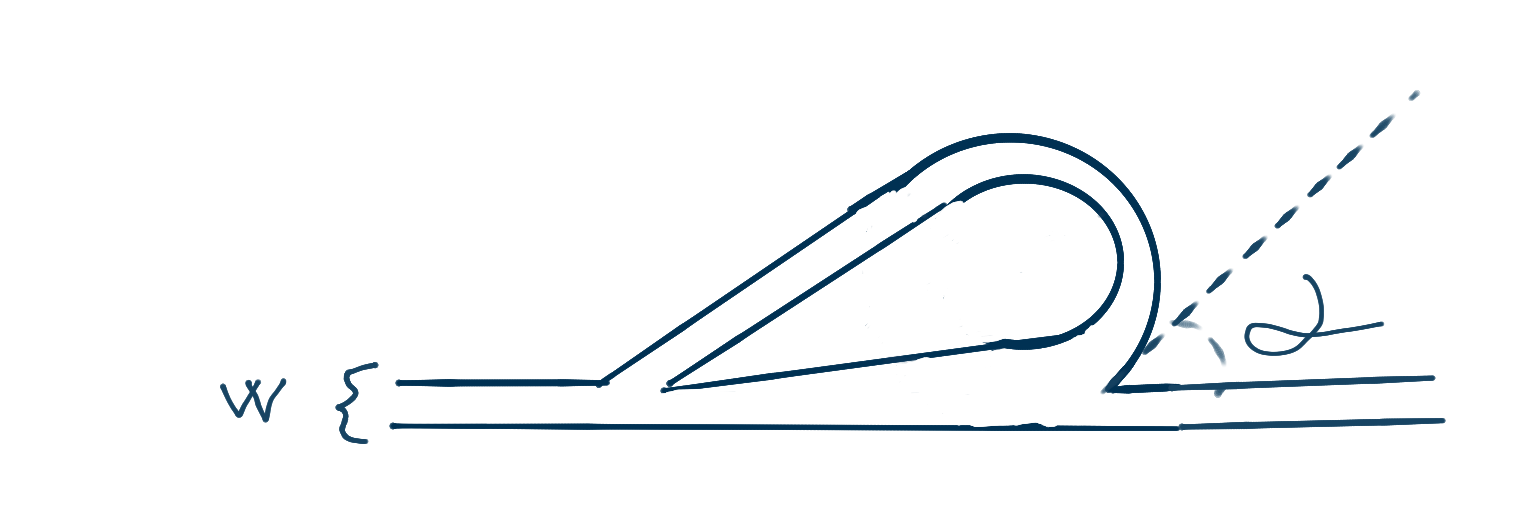
\includegraphics[width=100mm,scale=0.5]{teslaValve}
            \caption{Клапан Тесла.}
            \label{fig:TeslaValve}
        \end{figure}
        Это прямой канал с U-образным отводным каналом.
        Основной параметр для дальнейшего исследования -- это угол $ \alpha  $.
        
        На основе выбранного шаблона был написан скрипт для построения параметрической геометрии и расчетной сетки с минимальным количеством независимых параметров.
        
        \begin{figure}[h!]
            \centering
            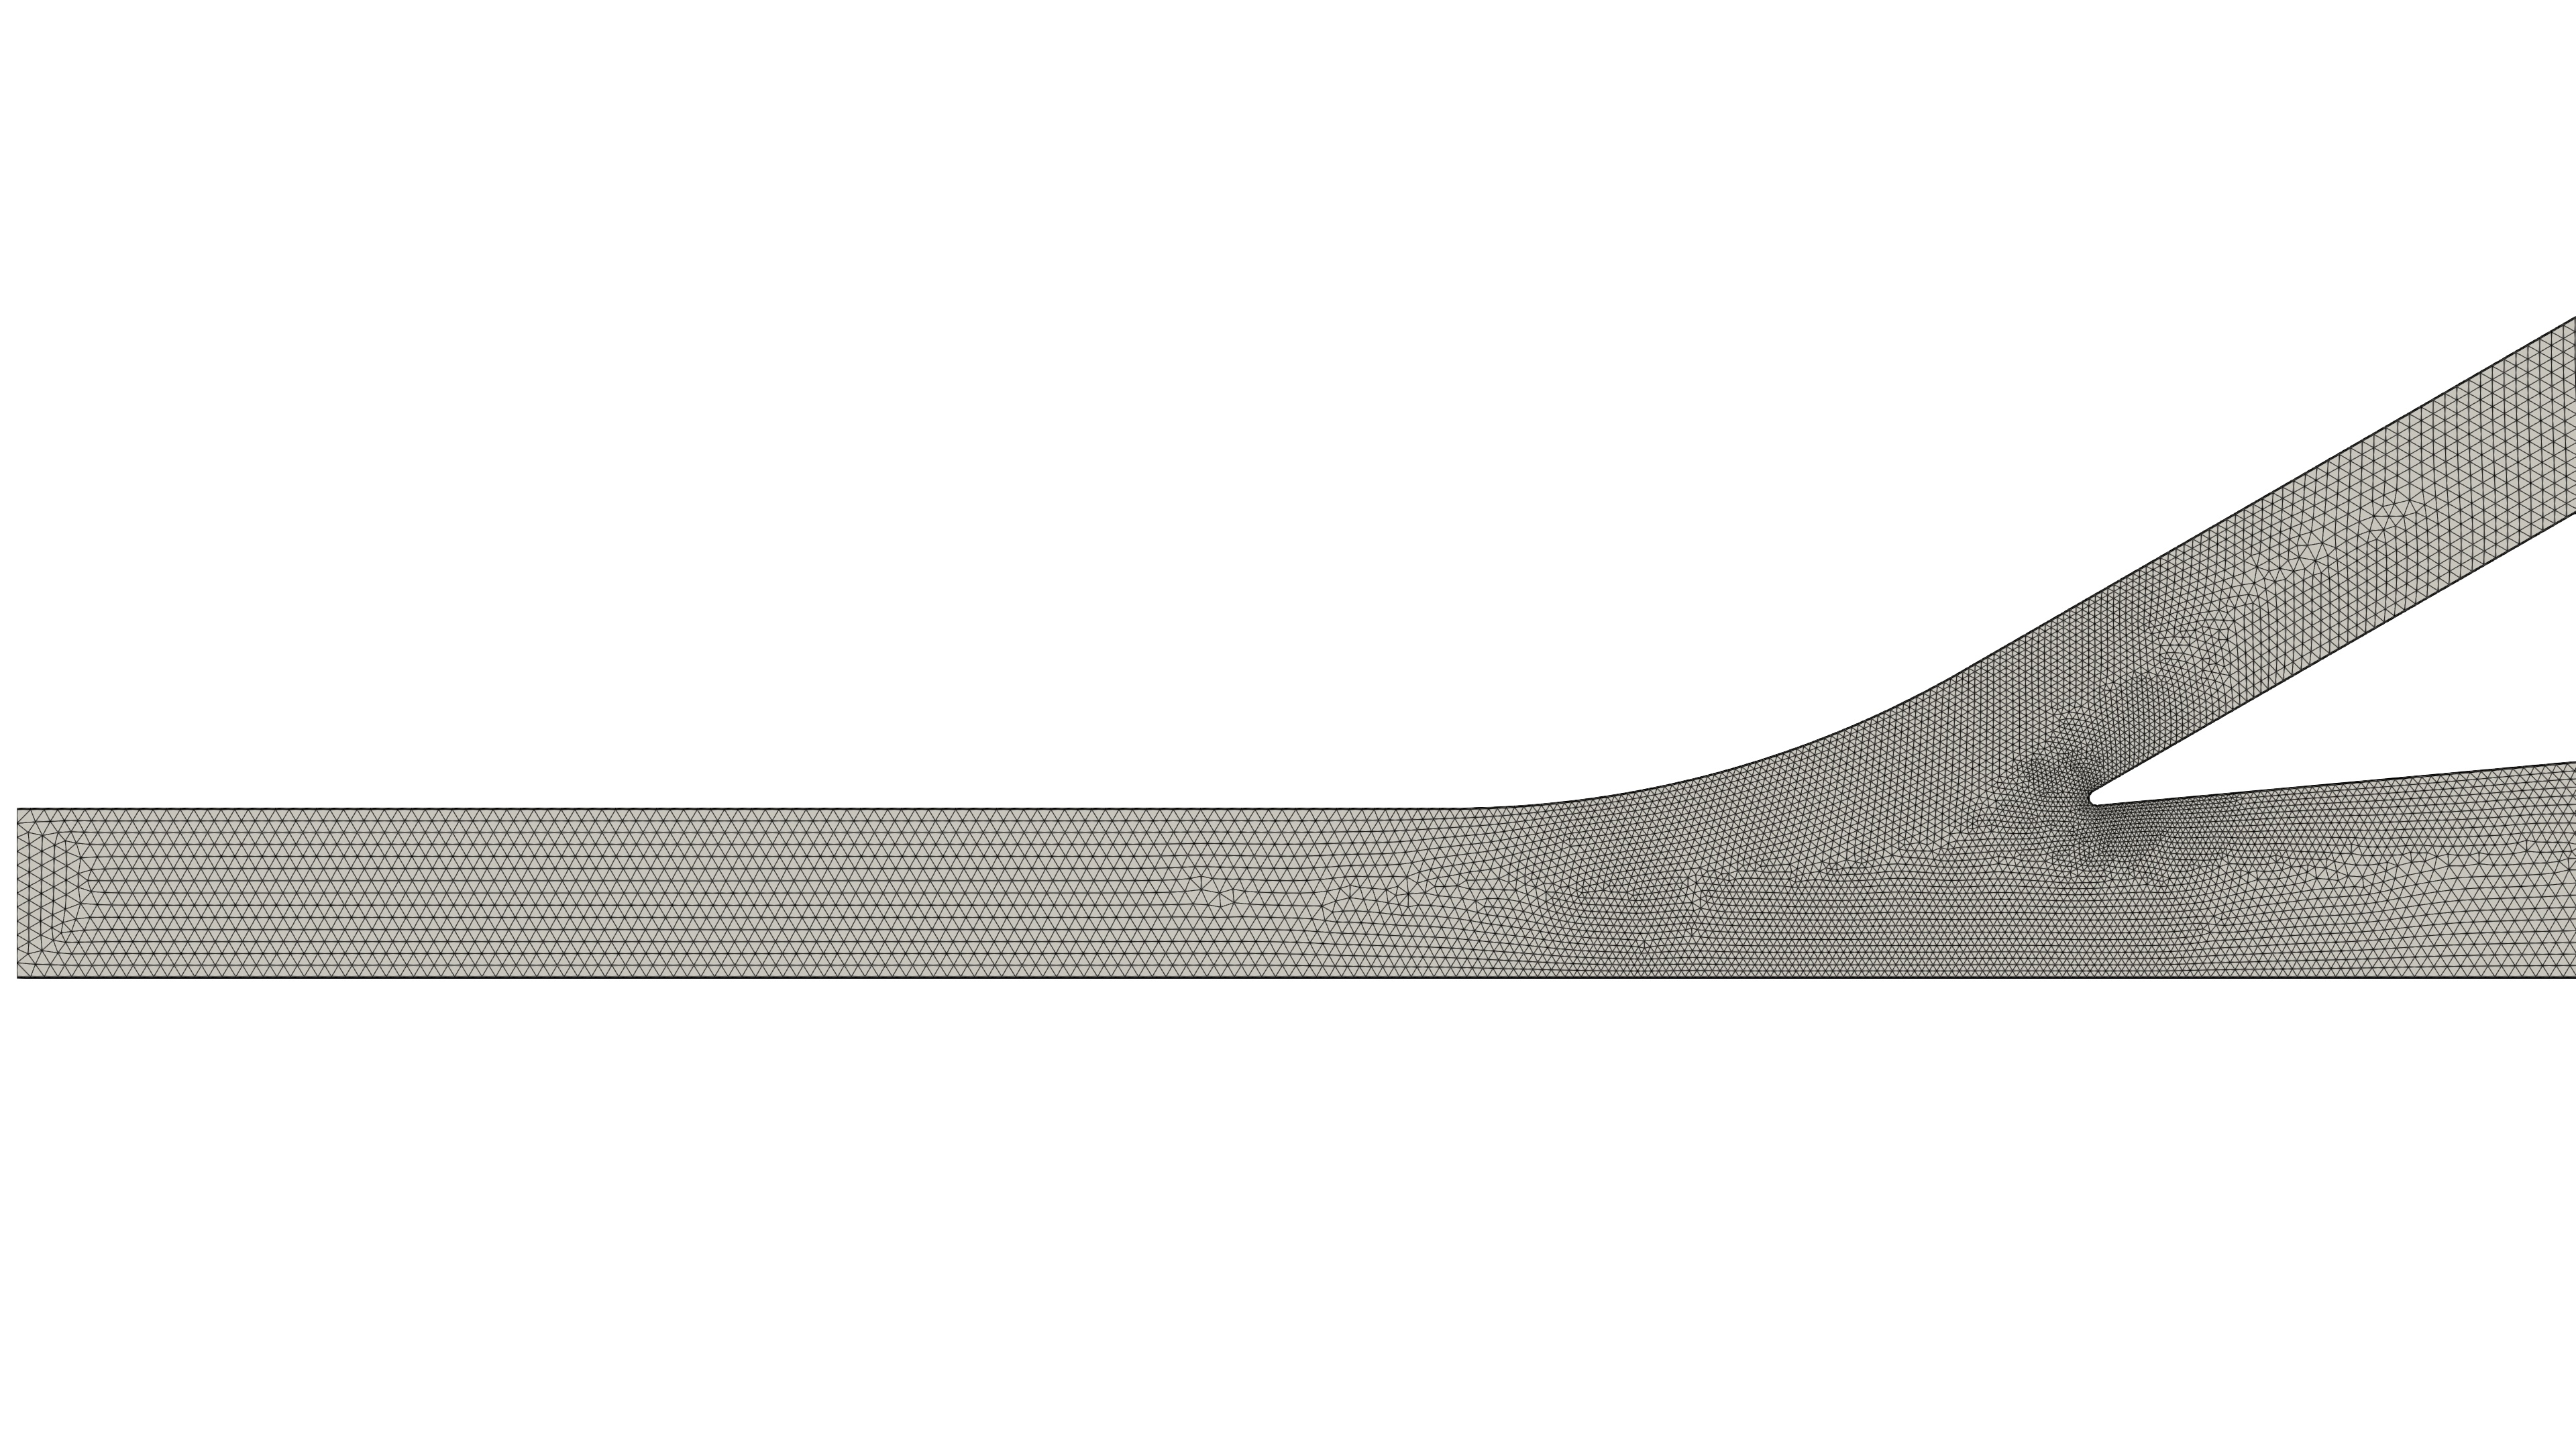
\includegraphics[width = 1\linewidth]{teslaMesh1}
            \caption{Расчетная сетка.}
            \label{fig:teslaMesh}
        \end{figure}
        
        На (рис.~\ref{fig:teslaMesh}) угол $\alpha$ равен 30 градусам. Также, можно видеть, что сетка не однородная и ее разрешение падает по мере удаления от зон с наибольшим интересом.
        
        \begin{figure}[H]
            \centering
            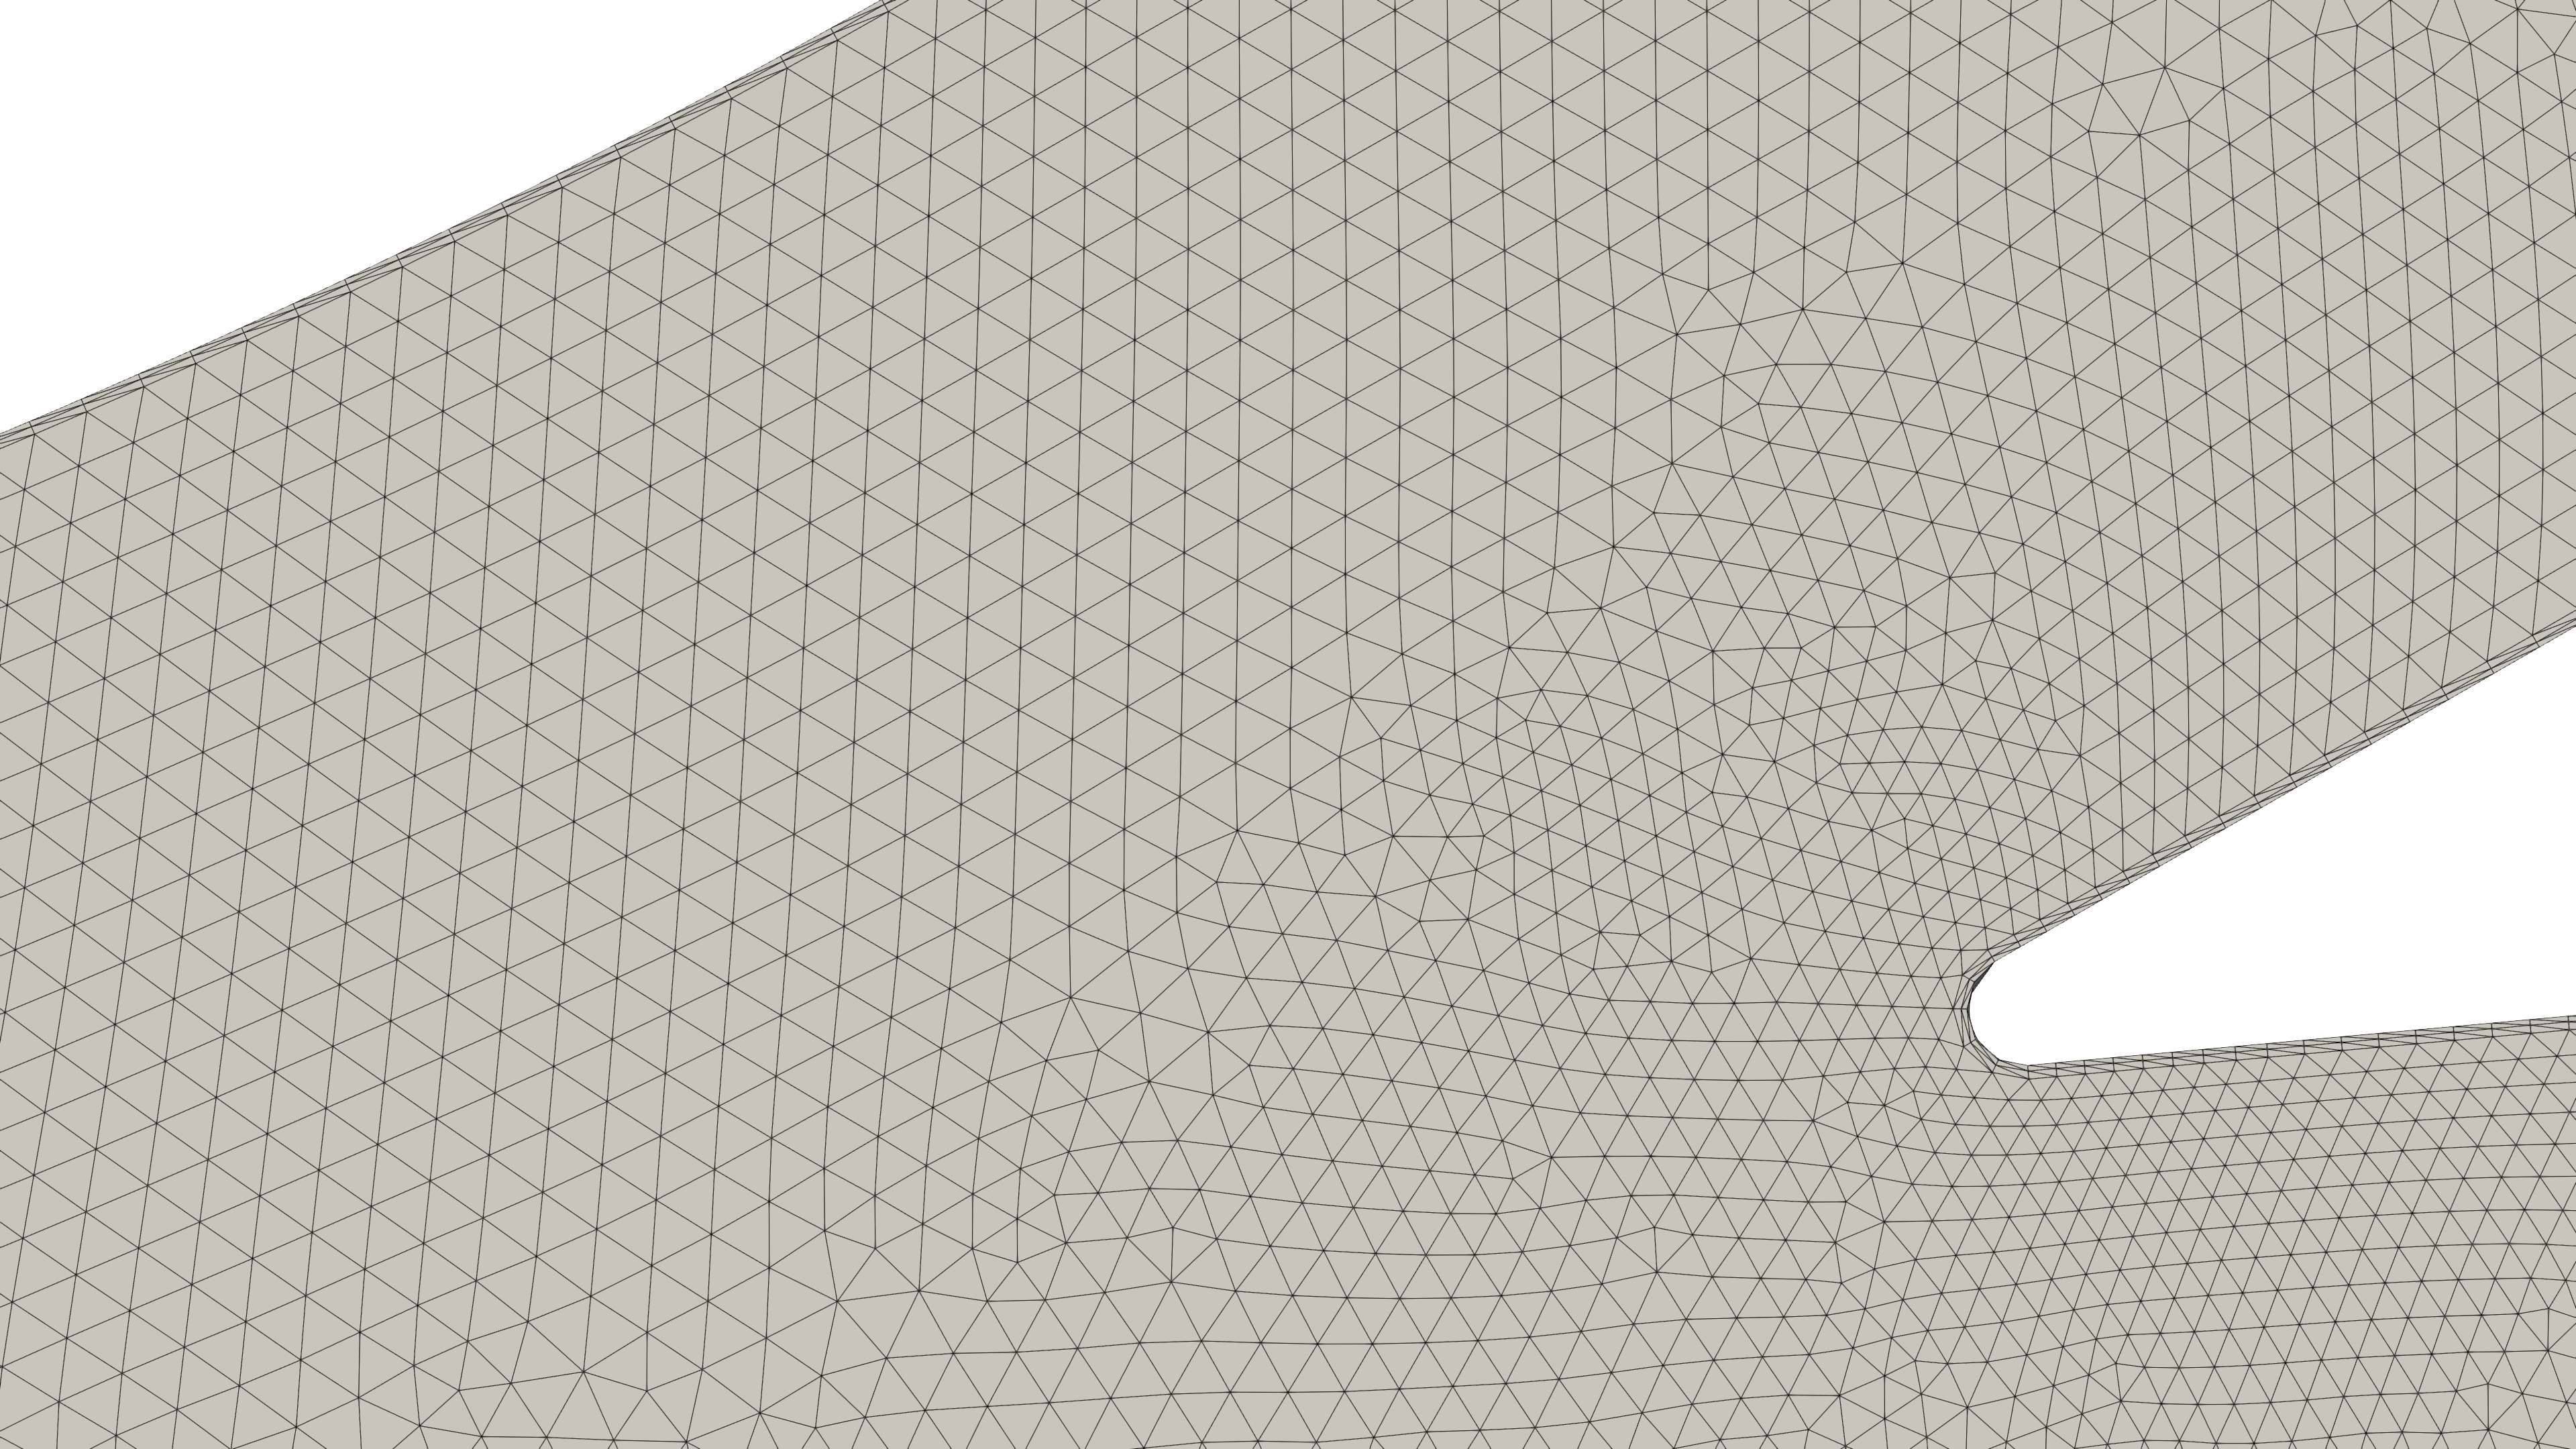
\includegraphics[width = 1\linewidth]{teslaMesh2}
            \caption{Расчетная сетка в приближении.}
            \label{fig:teslaMesh2}
        \end{figure}   
             
        Для разрешения градиента скорости вблизи стенок был добавлен сеточный подслой (рис.~\ref{fig:teslaMesh2}).
        
    \section*{Режим течения и расчет.}        
        
        Чтобы определить какого рода перед нами течение, можно рассчитать число Рейнольдса, Re. Исходя из полученного значения, можно будет сделать выводы о характере потока, турбулентное или ламинарное.
        Так как канал нашей конфигурации клапана Теслы имеет квадратное сечение, то формула для определения числа Рейнольдса имеет вид:
        
        \begin{equation}\label{eqn:Re}
            Re = \frac{u D_{H}}{\nu}
        \end{equation}
            
        Где  u - скорость в канале, м/с, $ D_{H} $ - гидравлический диаметр, м, $\nu$ - кинематическая вязкость, м$^{2}/$с. 
        
        $D_{H} = \frac{4A}{P}$,\\
        где A - площадь поперечного сечения канала, м$^{2}$, P - смоченный периметр. 
        
        Для нашей конфигурации скорость течения в канале будет равна 3 м/с, а число Рейнольдса - 1500. Ширина канала была выбрана равной 500 мкм или 0.0005 м.  
        
        Для числа Рейнольдса    
        
        OpenFoam - это открытый программный комплекс для решения задач механики сплошной среды. SimpleFoam - это стационарный решатель для несжимаемого турбулентного потока, использующий алгоритм SIMPLE. Математическая модель, реализованная в решателе simpleFoam, имеет вид:
        
        \begin{equation}\label{eqn:simpleFoam}
            \bm{\nabla} \cdot \bm{u} = 0
        \end{equation} 
        
        \begin{equation}\label{eqn:simpleFoam2}
            \bm{\nabla} \cdot \bm{u} \otimes \bm{u} = -\bm{\nabla} p + \bm{\nabla} \cdot \bm{\tau}
        \end{equation} 
        
        Где $\bm{u}$ - скорость, м/с, p - кинематическое давление, м$^{2}/$с$^{2}$, $\bm{\tau}$ - тензор напряжения. 
        Каждый цикл итерации влечет за собой сначала расчет промежуточного поля скорости, которое удовлетворяет линеаризованным уравнениям импульса для предполагаемого распределения давления: затем применяется принцип сохранения массы для настройки скоростей и давлений, так что все уравнения находятся в равновесии.
        
       По графику невязок (рис.~\ref{fig:DRLam}) видно, что, при расчете без использования модели турбулентности, решение является неустойчивым. 
        
        \begin{figure}[H]
            \centering
            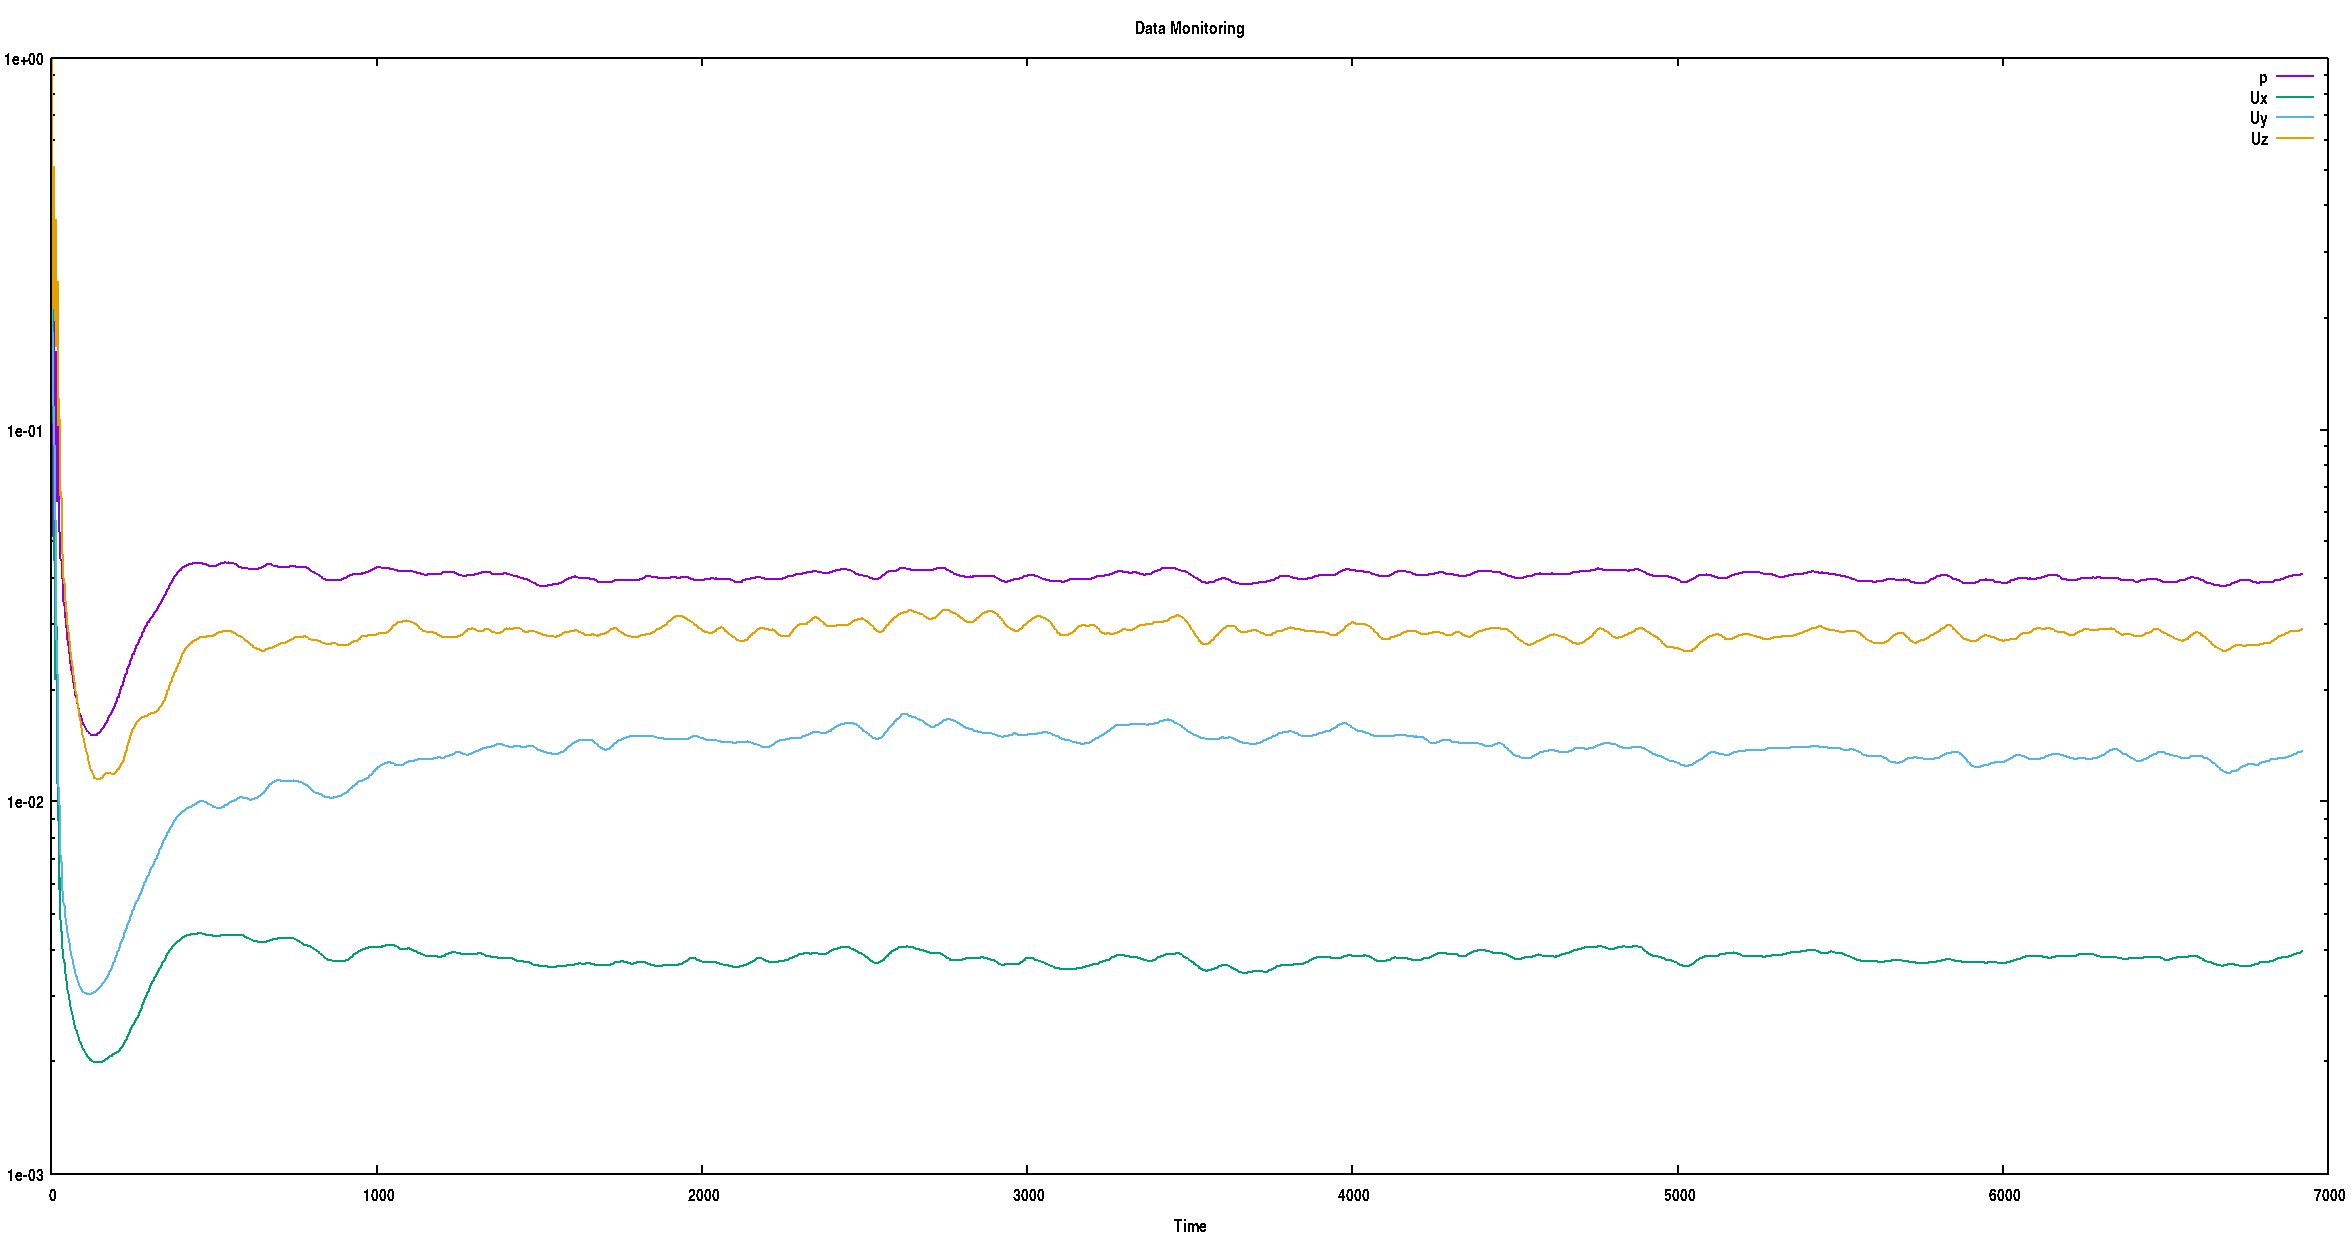
\includegraphics[width = 1\linewidth]{dataMonitoringLaminar}
            \caption{График невязок с ламинарной моделью.}
            \label{fig:DRLam}
        \end{figure}
        
        
        Исходя из этого было принято решение о подключении турбулентной модели k-epsilon. Выбранным типом моделирования турбулентности был параметр RAS. Модель k-epsilon объединяет уравнения турбулентной кинетической энергии (\ref{eqn:k}), k, и уравнение скорости рассеивания турбулентной кинетической энергии (\ref{eqn:e}), $\epsilon$.
        
        \begin{equation}\label{eqn:k}
            \frac{D}{D_{t}}(\rho k) = \nabla \cdot (\rho D_{k}\nabla k) + P - \rho\epsilon
        \end{equation} 
        
        \begin{equation}\label{eqn:e}
            \frac{D}{D_{t}}(\rho\epsilon) = \nabla \cdot (\rho D_{\epsilon}\nabla\epsilon) + \frac{C_{1}\epsilon}{k}(P + C_{3}\frac{2}{3}k\nabla \cdot \bm{u}) - C_{2}\rho\frac{\epsilon^2}{k}
        \end{equation} 
       Где k --- турбулентная кинетическая энергия, м$^2$/с$^2$, $D_{k}$ - Эффективная диффузионная способность для k, P - скорость производства турбулентной кинетической энергии, м$^2$/с$^-3$, $\epsilon$ - скорость рассеивания турбулентной кинетической энергии, м$^2$/с$^-3$, $D_{\epsilon}$ - Эффективная диффузионная способность для $\epsilon$.
               
        Далее решается уравнение для турбулентной вязкости:
        
        \begin{equation}\label{eqn:mu}
           \nu_{t} = C_{\mu}\frac{k^2}{\epsilon}
        \end{equation} 
        Где $C_{\mu}$ - модельный коэффициент турбулентной вязкости, $\mu_{t}$ - турбулентная вязкость, м$^2$/с$^-1$.
        
        \begin{figure}[H]
            \centering
            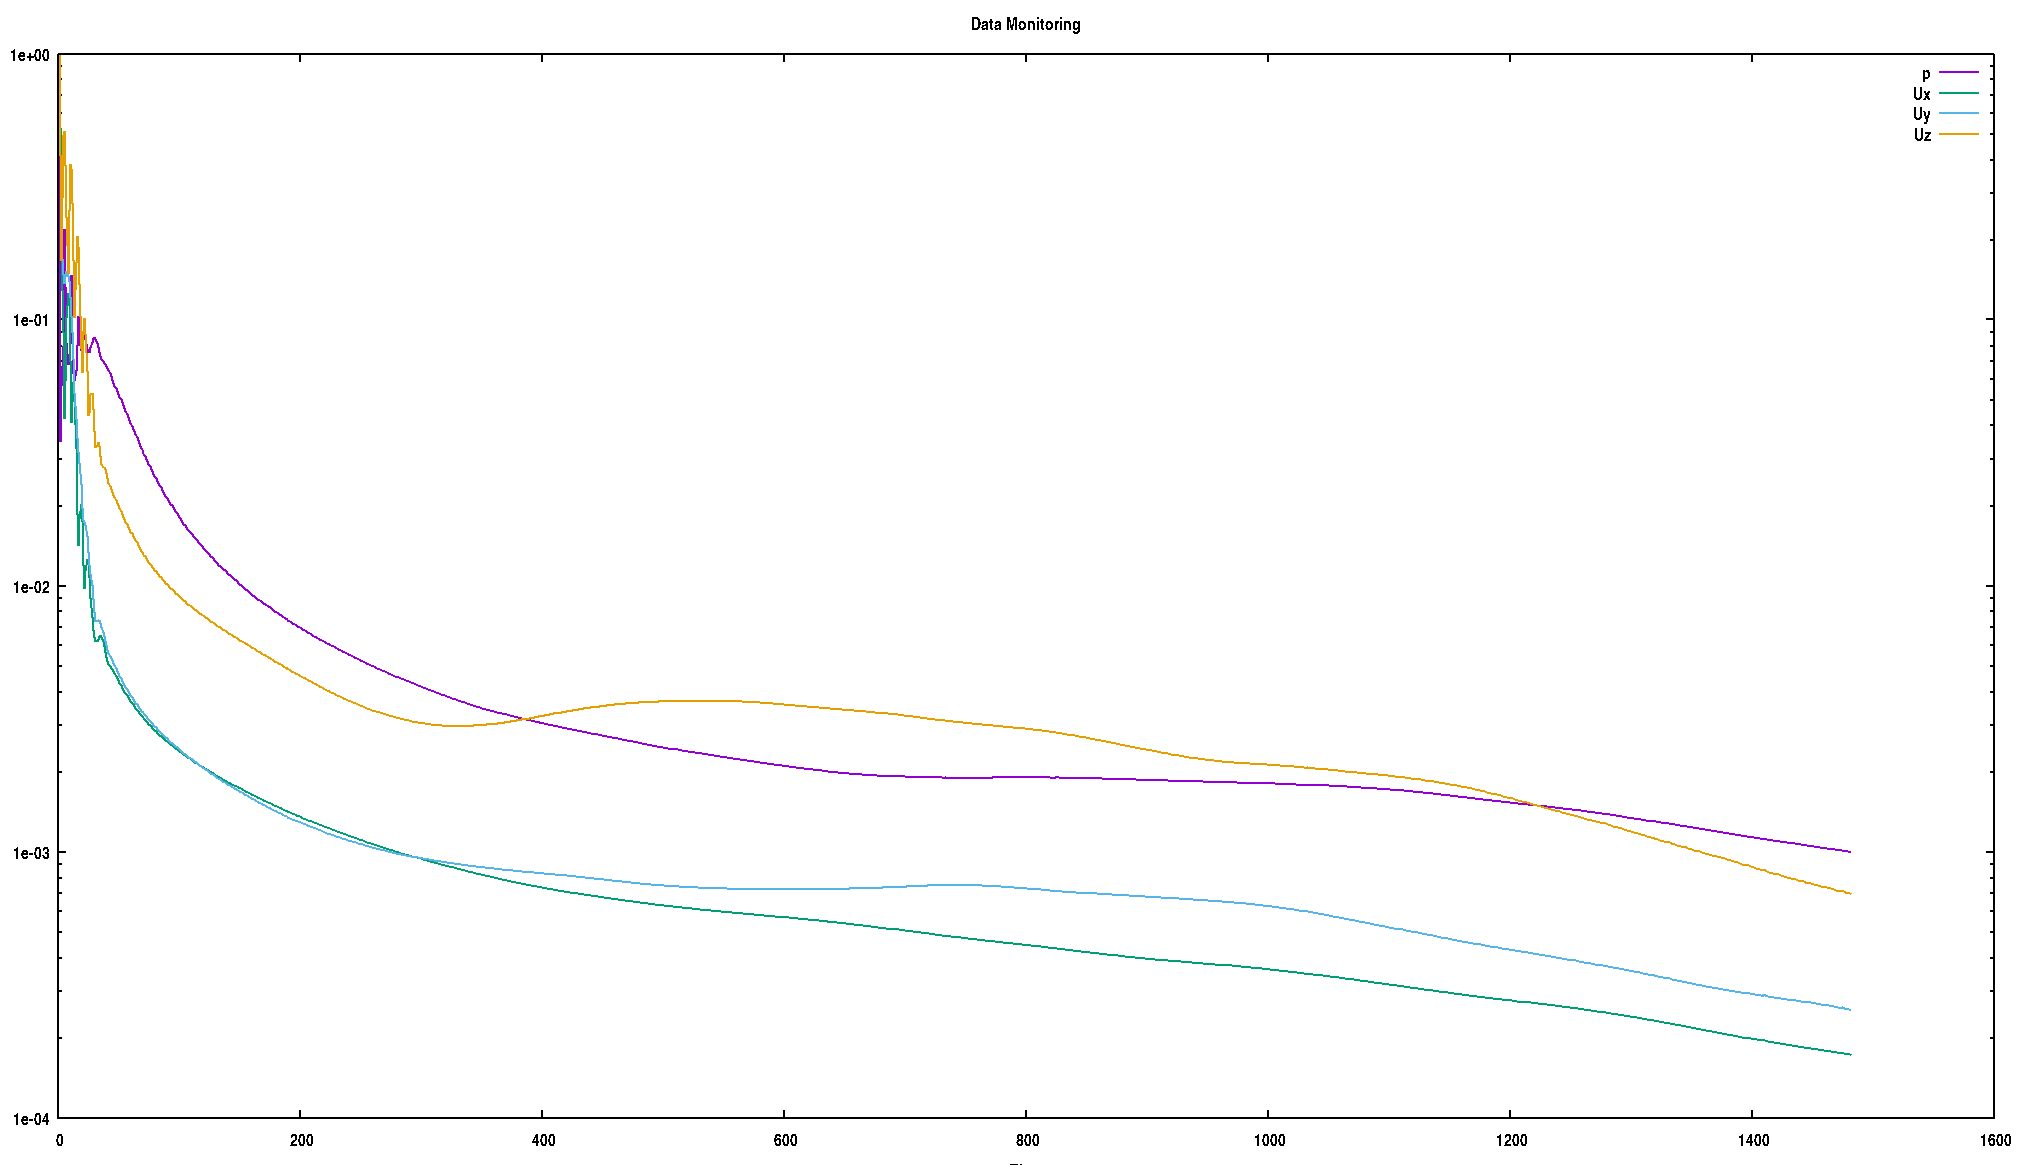
\includegraphics[width = 1\linewidth]{dataMonitoringRAS}
            \caption{График невязок с моделью турбулентности.}
            \label{fig:DRRAS}
        \end{figure}
        
        Граничные условия. Для решения уравнений турбулентности заданы через интенсивность для k (\ref{eqn:kI}) и через длину перемешивания для $\epsilon$ (\ref{eqn:el}). Граничные условия для скорости заданы через объемный расход, для давления через абсолютное давление (\ref{eqn:P0}).
        
        \begin{equation}\label{eqn:kI}
            k_{p} = 1.5 (I |U|)^2
        \end{equation}
        Где $k_{p}$ - кинетическая энергия на границе, м$^2$/с$^2$, I - интенсивность турбулентности.
        
        \begin{equation}\label{eqn:el}
            \epsilon_{p} = \frac{C_{\mu}^{0.75} k^{1.5}}{L}           
        \end{equation}
        Где $\epsilon_{p}$ - диссипация кинетической энергии на границе, м$^2$/с$^-3$, L - шкала длины.
        
        \begin{equation}\label{eqn:P0}
            p_{p} = p_{0} + \frac{1}{2}\ \left|u_{0}\right|^2 - \frac{1}{2}\ \left|u\right|^2
        \end{equation}
        Где $p_{p}$ - давление на границе, м$^{2}/$с$^{2}$, $p_{0}$ - внешнее статическое давление, м$^{2}/$с$^{2}$, $u$ - скорость, м/с, $u_{0}$ - внешняя скорость, м/с.
        
        Оценка полученных результатов. Для оценки эффективности клапана Тесла, оценим его диодность, Di (\ref{eqn:Di}). Если Di > 1, то рассматриваемый клапан можно считать рабочим. Для этого мы проводили расчет нашей конфигурации клапана Тесла с одинаковыми параметрами дважды, но при разных подключениях: при обратном, когда перепад давления наибольший, и, при прямом, когда перепад давления наименьший. Полученные данные фиксировались.         
        
        \begin{equation}\label{eqn:Di}
            Di = (\frac{\bigtriangleup p_{r}}{\bigtriangleup p_{f}})_Q
        \end{equation}
        Где $\bigtriangleup p_{r}$ - перепад давления при обратном подключении, $\bigtriangleup p_{f}$ - перепад давления при прямом подключении для скорости потока Q.
        
        \section*{Результаты.}
        
        
    
\end{document}    